\documentclass[12pt,letterpaper]{article}
\usepackage{graphicx,textcomp}
\usepackage{natbib}
\usepackage{setspace}
\usepackage{fullpage}
\usepackage{fancyvrb}
\usepackage{color}
\usepackage[reqno]{amsmath}
\usepackage{amsthm}
\usepackage{amssymb,enumerate}
\usepackage[all]{xy}
\usepackage{endnotes}
\usepackage{lscape}
\usepackage{float}
\newtheorem{com}{Comment}
\newtheorem{lem} {Lemma}
\newtheorem{prop}{Proposition}
\newtheorem{thm}{Theorem}
\newtheorem{defn}{Definition}
\newtheorem{cor}{Corollary}
\newtheorem{obs}{Observation}
\usepackage[compact]{titlesec}
\usepackage{dcolumn}
\usepackage{tikz}
\usetikzlibrary{arrows}
\usepackage{multirow}
\usepackage{xcolor}
\newcolumntype{.}{D{.}{.}{-1}}
\newcolumntype{d}[1]{D{.}{.}{#1}}
\definecolor{light-gray}{gray}{0.65}
\usepackage{url}
\usepackage{listings}
\usepackage{color}
 
\definecolor{codegreen}{rgb}{0,0.6,0}
\definecolor{codegray}{rgb}{0.5,0.5,0.5}
\definecolor{codepurple}{rgb}{0.58,0,0.82}
\definecolor{backcolour}{rgb}{0.95,0.95,0.92}
 
\lstdefinestyle{mystyle}{
    backgroundcolor=\color{backcolour},   
    commentstyle=\color{codegreen},
    keywordstyle=\color{magenta},
    numberstyle=\tiny\color{codegray},
    stringstyle=\color{codepurple},
    basicstyle=\footnotesize,
    breakatwhitespace=false,         
    breaklines=true,                 
    captionpos=b,                    
    keepspaces=true,                 
    numbers=left,                    
    numbersep=5pt,                  
    showspaces=false,                
    showstringspaces=false,
    showtabs=false,                  
    tabsize=2
}
 \lstset{style=mystyle}
\newcommand{\Sref}[1]{Section~\ref{#1}}
\newtheorem{hyp}{Hypothesis}

\title{Text as Data: Homework 3}
\date{August 17, 2017}
\author{Jeff Ziegler}

\begin{document}
\maketitle

In this homework we will analyze a collection of news stories from the New York Times from the November 1-3, 2004 (the day before, of, and after the 2004 general election). This data come from the New York Times Annotated Corpus and is for academic use only. We have done some preprocessing in order to simplify the homework tasks.


\section{Preprocessing and Creating a Document-Term Matrix}

\begin{itemize}
\item[a)] From the course github, download {\tt nyt\_ac.json} 
\item[b)] Using the {\tt JSON} library in python, import the data. Use {\tt type} to explore the structure of this data. How are this data organized?
\item[c)] Extract the title and text from each story.  Create an individual document for each story and write each of the files to a new directory 
\item[d)] Using the loaded {\tt json} file, create a document term matrix of the 1000 most used terms.  Be sure to: 
\begin{itemize}
\item[-] Discard word order
\item[-] Remove stop words
\item[-] Apply the porter stemmer
\end{itemize}
\item[e)] Include in your document-term matrix the \emph{desk} from which the story originated, which we will include later
\end{itemize}

\lstinputlisting[language=Python, firstline=5, lastline=36]{WUSTL_HW3_JZ.py}

\begin{Verbatim}
['0.txt',
 '1.txt',
 '10.txt',
 '100.txt',
 '101.txt',
 '102.txt',
 '103.txt',
 ...]
\end{Verbatim}

\lstinputlisting[language=Python, firstline=37, lastline=126]{WUSTL_HW3_JZ.py}

\subsection*{Clustering Methods}

\begin{itemize}
\item[1)] Using the {\tt kmeans} function, create a plot of the {\tt kmeans} objective function as the number of clusters varies from 2 to $N - 1$.  
\end{itemize}
  
\lstinputlisting[language=R, firstline=1, lastline=30]{WUSTL_HW3_JZ.r}  
  
\begin{figure}[H]
  \caption{\footnotesize{{\tt kmeans} objective function as number of clusters varies.}}
  \centering
   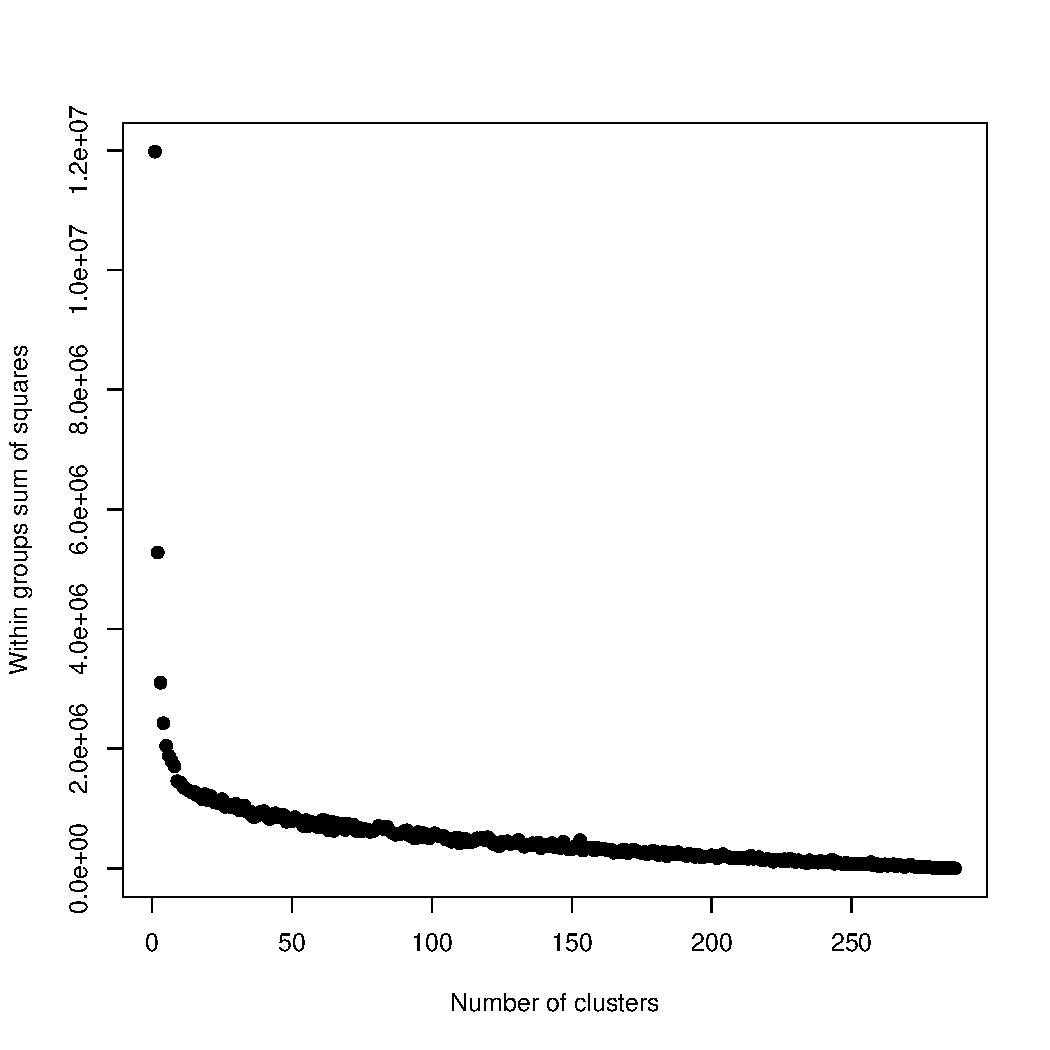
\includegraphics[width=.7\linewidth]{HW3kmeansClusters.pdf}\\
\end{figure}
  
  
 \begin{itemize}
\item[2)] Apply K-Means with 6 clusters, being sure to use {\tt set.seed} to ensure you can replicate your analysis
\item[3)] Label each cluster using computer and hand methods:
\begin{itemize}
\item[i)] Suppose $\boldsymbol{\theta}_{k}$ is the cluster center for cluster $k$ and define $\bar{\boldsymbol{\theta}}_{-k} = \frac{\sum_{j \neq k} \boldsymbol{\theta_{j}}   }{K-1 }$ or the average of the centers not $k$.  Define 
\begin{eqnarray}
\text{Diff}_{k} & = & \boldsymbol{\theta}_{k} - \bar{\boldsymbol{\theta}}_{-k}\nonumber 
\end{eqnarray}

\lstinputlisting[language=R, firstline=31, lastline=68]{WUSTL_HW3_JZ.r}  

Use the top ten words from $\text{Diff}_{k}$ to label the clusters
\item[ii)] Sample and read texts assigned to each cluster and produce a hand label
\end{itemize}
\end{itemize}

\lstinputlisting[language=R, firstline=70, lastline=82]{WUSTL_HW3_JZ.r}  

\begin{Verbatim}[fontsize=\footnotesize]
[1] ""title": "Red-Zone Forays Put Giants in the Black",
"body_text": "The Giants did not exactly become an offensive 
juggernaut in Sunday's victory over Minnesota. They gained
283 yards, collected 83 yards in penalties from the Vikings and 
absorbed five sacks, and quarterback Kurt Warner fumbled 
three snaps... <truncated>
[2]""title": "G.O.P. in Ohio Can Challenge Voters at Polls", 
"body_text": "In a day of see-sawing court rulings, a Federal appeals 
court ruled early Tuesday morning that the Republican Party could 
place thousands of people inside polling places to challenge the
eligibility of voters, a blow to Democrats who argued those challengers
 will intimidate minority voters... <truncated>
\end{Verbatim}

\section{Dictionary Classification Methods}
\begin{itemize}
\item[a)] Download the list of positive (http://www.unc.edu/~ncaren/haphazard/positive.txt) and negative (http://www.unc.edu/~ncaren/haphazard/negative.txt) stop words from Neil Caren's website.
\item[b)] Calculate a positive score and a negative score for each document and the difference between each score using the dictionaries
\end{itemize}

\lstinputlisting[language=Python, firstline=128, lastline=200]{WUSTL_HW3_JZ.py}

\begin{itemize}
\item[c)] How does the score change before and after the election?  How does the score vary across desks?
\end{itemize}

\lstinputlisting[language=R, firstline=84, lastline=100]{WUSTL_HW3_JZ.r}  

\begin{table}[H] \centering 
  \caption{Regression results of sentimental change.} 
  \label{} 
\begin{tabular}{@{\extracolsep{5pt}}lcc} 
\\[-1.8ex]\hline 
\hline \\[-1.8ex] 
 & \multicolumn{2}{c}{\textit{Dependent variable:}} \\ 
\cline{2-3} 
\\[-1.8ex] & NposPorter & NnegPorter \\ 
\\[-1.8ex] & (1) & (2)\\ 
\hline \\[-1.8ex] 
Election day & $-$0.003 & $-$0.001 \\ 
  & (0.002) & (0.002) \\ 
Day after election & 0.001 & $-$0.002 \\ 
  & (0.002) & (0.002) \\ 
 Editorial Desk & 0.013$^{***}$ & 0.015$^{***}$ \\ 
  & (0.004) & (0.003) \\ 
 Foreign Desk & $-$0.005 & 0.013$^{***}$ \\ 
  & (0.003) & (0.003) \\ 
 Health and Fitness & 0.016$^{***}$ & 0.011$^{**}$ \\ 
  & (0.006) & (0.005) \\ 
 Metropolitan Desk & $-$0.001 & 0.010$^{*}$ \\ 
  & (0.006) & (0.006) \\ 
 National Desk & 0.003 & 0.007$^{***}$ \\ 
  & (0.002) & (0.002) \\ 
 Science Desk & 0.002 & 0.001 \\ 
  & (0.006) & (0.006) \\ 
 Sports Desk & 0.002 & $-$0.0002 \\ 
  & (0.003) & (0.003) \\ 
 The Arts/Cultural Desk & 0.011$^{***}$ & 0.005$^{**}$ \\ 
  & (0.003) & (0.003) \\ 
 Constant & 0.054$^{***}$ & 0.033$^{***}$ \\ 
  & (0.002) & (0.002) \\ 
\hline \\[-1.8ex] 
Observations & 288 & 288 \\ 
R$^{2}$ & 0.144 & 0.144 \\ 
\hline 
\hline \\[-1.8ex] 
\textit{Note:}  & \multicolumn{2}{r}{$^{*}$p$<$0.1; $^{**}$p$<$0.05; $^{***}$p$<$0.01} \\ 
\end{tabular} 
\end{table} 

\section{Supervised Learning with Naive Bayes}

\begin{itemize}
\item[a)] Using the version of Naive Bayes outlined on slide 24 of lecture 14, write a function to estimate $p(C_{k})$ and $\boldsymbol{\theta}_{k}$ for an arbitrary collection of categories.  Hint: to compute the probability of a document from a category, note you can work with the log of the probability equivalently.  
\item[b)] Let's focus on documents that came from Business/Financial desk and National Desk.  Using leave-one out cross validation, calculate the accuracy of Naive Bayes to calculate the label.
\item[c)] Compare the performance of Naive Bayes to the performance of 2 of the following 3 algorithms using 10-fold cross validation:
\begin{itemize}
\item[-] LASSO 
\item[-] Ridge 
\item[-] KRLS 
\end{itemize}
How does Naive Bayes compare? 
\end{itemize}

\lstinputlisting[language=R, firstline=102]{WUSTL_HW3_JZ.r}  

\end{document}
